\newcommand{\D}{\mathcal{D}}
\newcommand{\bc}[2]{\ensuremath{[\,#1\,\vdash #2\,]}}
\newcommand{\sof}{\ensuremath{\!:\ms}}
\newcommand{\ssep}{\ensuremath{,\ms}}

The programming and proof environment Beluga~\cite{Pientka:FLOPS10,Pientka:CADE15} is another system that supports HOAS.
Object languages are encoded in the logical framework LF~\cite{Harper93jacm}, while proofs about these are expressed as total programs in contextual modal type theory, Beluga's reasoning logic.
The programs analyse LF derivation trees using pattern matching and higher-order unification.
In Beluga, it is necessary to give programs (i.e.\ proof terms) explicitly, which are proof checked as part of type checking.
This stands in contrast to Coq and Abella, both of which are interactive systems with a tactic language for proof term construction.

\enlargethispage{\baselineskip}

The biggest difference, however, lies with Beluga's treatment of object level variables.
In particular, at the outermost level, there is no such thing as a free object variable.
This is in stark contrast to Coq's dangling de Bruijn indices and Abella's global nominal constants.
In Beluga we instead deal with \emph{contextual objects}, written $\bc{\Gamma}{K}$, that is objects $K$ (like types, terms, typing derivations) paired with contexts $\Gamma$ in which they are meaningful~\cite{Nanevski:ICML05,Pientka:POPL08}.

As an example, consider the function type $X \to X$ where $X$ is a free type variable.
This function type is ill-formed under the empty type variable context $\Delta = \emptyset$.
In Coq and Abella we can express this type, as $0_\ty \to 0_\ty$ and respectively $n_0 \to n_0$.
We can then show that assuming well-formedness under the empty context entails absurdity, $\istyF{0}{0_\ty \to 0_\ty} \implies \bot$ and $\aj{\emptyctx}{\istyFh{n_0 \to n_0}} \implies \bot$.
Meanwhile in Beluga, we observe that the contextual object $\bc{\emptyctx}{x \to x}$ is not even syntactically well-formed, since $x \notin \emptyctx$.
An immediate consequence of this is that the type formation judgement for F, which ensures that the context is covering all free type variables, becomes redundant.
Hence Beluga's definition of F is obtained from Figure~\ref{fig:sys-f-abella} by removing all references to type formation.
The definition of \SysL is identical to the one for Abella (Figure\ref{fig:sys-l-abella}).

Recall that context management was completely manual in Coq.
Each judgement required well-chosen generalisations and custom invariants to accurately track contextual information.
In Abella the situation was noticeably better, as contexts at the object level were kept implicit and handled by the system.
At the reasoning level they did, however, surface as explicit, unstructured sequences of judgements.
The desired contextual structure then had to be imposed with auxiliary predicates, together with copious amounts of inversion lemmas.

Beluga contexts, on the other hand, are sequences of not necessarily homogeneous declarations.
Each declaration can depend on prior declarations and encapsulate multiple pieces of related information using a dependent record.
Contexts are first class citizens and \emph{context schema} ascription, $\Gamma \OF S$, is used to ensure that a given context $\Gamma$ satisfies certain structural constraints.

Schemas are Beluga's main device to enforce invariants on contextual information.
We use propagation for \SysL as an example.
The requisite schema is:
\begin{align*}
  S_{\lambda W} \eqdef [x\sof\TmL \ssep \typingLh{x}{\Prp}] + [x\sof\TmL \ssep \typingLh{x}{a} \ssep \typingLh{a}{\Prp}]
\end{align*}

Note how it separates PTS variables into type and term variables via the associated typing information, which already imposes the necessary semantic contextual information.
The proof of propagation is straightforward.
We implement a total recursive function $k$ satisfying:
\begin{align*}
  k \OF \mAll{\Gamma \of S_{\lambda W}} \bc{\Gamma}{\typingLh{a}{b}} \implies \bc{\Gamma}{\mathsf{type\_correct}\,b}
\end{align*}

The contextual predicate $\bc{\Gamma}{\mathsf{type\_correct}\,b}$ encodes that $b$ is either $\Typ$ or it can be typed with some universe $u$.
We pattern match $\D \OF \bc{\Gamma}{\typingLh{a}{b}}$ and obtain seven cases.
The first four are structural, recursively descending into sub-derivations.
The only part that is non-obvious is the traversal of binders, where various pieces of information are added to the context.
These have to be packaged into declaration blocks in order to satisfy $S_{\lambda W}$ for the recursive call.
More interesting though are the three base cases.
When we compare the matched type against $S_{\lambda W}$, we observe three ways in which $\D$ could have been obtained from the context.
The first and third are trivial as they unify $b$ with $\Prp$ which can be typed with the universe $\Typ$.
For the remaining case we know that $b$ can be typed with the universe~$\Prp$, contextual information that was packaged together with the matched judgement.
Note that throughout the construction we exploit that Beluga natively supports substitution into parametric sub-derivations.

{\bf The third equivalence proof.}
The definitions of $\tyr$ and $\tmr$ exactly coincide with Abella.
We are going to primarily concern ourselves with the schemas, which best illustrate Beluga's tracking of contextual information.

We begin with the functionality and injectivity properties of $\tyr$ and $\tmr$.
Since equality is not native in Beluga we have to define equality predicates for each syntactic sort to express our statements. The tightest invariants that hold for the rules defining $\tyr$ and $\tmr$ can be expressed with the following context schemas:
\begin{align*}
  S_{\tyr} &\eqdef [x\sof\TyF \ssep y\sof\TmL \ssep x \tyr y] + [y\sof\TmL]\\
  S_{\tmr} &\eqdef [x\sof\TyF \ssep y\sof\TmL \ssep x \tyr y] + [x\sof\TmF \ssep y\sof\TmL \ssep x \tmr y]
\end{align*}

Due to the subordination ordering of $\tyr$ and $\tmr$, Beluga is capable of automatically strengthening from $S_{\tmr}$ to $S_{\tyr}$, and weaken vice versa (see also~\cite{Virga99phd}).
\begin{lemma}
  There exist total recursive functions $f_{\ty}, f_{\tm}, i_{\ty}$ and $i_{\tm}$, satisfying
  \begin{align*}
    f_{\ty} &\OF  \mAll{\Gamma \of S_{\tyr}} \bc{\Gamma}{A \tyr a} \implies \bc{\Gamma}{A \tyr a'} \implies \bc{\Gamma}{a =_{\lambda} a'}\\
    i_{\ty} &\OF  \mAll{\Gamma \of S_{\tyr}} \bc{\Gamma}{A \tyr a} \implies \bc{\Gamma}{A' \tyr a} \implies \bc{\Gamma}{A =^{\ty}_{\mathsf{F}} A'}\\
    f_{\tm} &\OF  \mAll{\Gamma \of S_{\tmr}} \bc{\Gamma}{s \tmr a} \implies \bc{\Gamma}{s \tmr a'} \implies \bc{\Gamma}{a =_{\lambda} a'}\\
    i_{\tm} &\OF  \mAll{\Gamma \of S_{\tmr}} \bc{\Gamma}{s \tmr a} \implies \bc{\Gamma}{s' \tmr a} \implies \bc{\Gamma}{s =^{\tm}_{\mathsf{F}} s'}
\end{align*}
\end{lemma}
\begin{proof}
  Each by induction on the first premise and pattern matching on the second.
  In the variable cases we have matched against two context records $r$ and $r'$.
  Since $x$ and $y$ are local to $r$ and one of them is shared between the two matched records, unification infers $r = r'$, closing the case.
  Note that $f_{\tm}$ and $i_{\tm}$ contain calls to $f_{\ty}$ and respectively $i_{\ty}$, which relies on context strenghtening.
  For $i_{\tm}$ we also again require disjointedness of the two relations, which is easily obtainable under contexts satisfying $S_{\tmr}$.
\end{proof}

For the remaining four totality and preservation proofs we have to deal with two complications.
First, we have to remove assumptions and conclusions referring to F type formation.
Second, we have to define predicates that capture the existential nature of the four conclusions, including relevant typing information, with custom predicates.
We have, for example,
\begin{align*}
  \mathsf{exists\_rel\_proof}\,s\,A \iff \mEx{ba} s \tmr b \mAnd A \tyr a \mAnd \typingLh{b}{a} \mAnd \typingLh{a}{\Prp}
\end{align*}
The required context schemas are quite involved:
\begin{align*}
  S_{\tyr W}^{\rightarrow} \eqdef &[x\sof\TyF \ssep y\sof\TmL \ssep x \tyr y \ssep \typingLh{y}{\Prp}] + [y\sof\TmL \ssep \typingLh{y}{a}]\\
  S_{\tyr W}^{\leftarrow} \eqdef &[x\sof\TyF \ssep y\sof\TmL \ssep x \tyr y \ssep \typingLh{y}{\Prp}] + [y\sof\TmL \ssep \typingLh{y}{a} \ssep A \tyr a \ssep \typingLh{a}{\Prp}]\\
  S_{\tmr W} \eqdef &[x\sof\TyF \ssep y\sof\TmL \ssep x \tyr y \ssep \typingLh{y}{\Prp}] + [x\sof\TmF \ssep y\sof\TmL \ssep x \tmr y \ssep \typingFh{x}{A} \ssep \typingLh{y}{a} \ssep A \tyr a]
\end{align*}
\begin{lemma}
  There exist total recursive functions $p^{\rightarrow}_{\tyr},p^{\leftarrow}_{\tyr},p^{\rightarrow}_{\tmr}$ and $p^{\leftarrow}_{\tmr}$, satisfying
  \begin{align*}
    p^{\rightarrow}_{\tyr} &\OF  \mAll{\Gamma \of S_{\tyr}^{\rightarrow}} \mAll{A \of \bc{\Gamma}{\TyF}} \bc{\Gamma}{\mathsf{exists\_rel\_prop}\,A}\\
    p^{\leftarrow}_{\tyr} &\OF \mAll{\Gamma \of S_{\tyr}^{\leftarrow}} \bc{\Gamma}{\typingLh{a}{\Prp}} \implies \bc{\Gamma}{\mathsf{exists\_rel\_type}\,a}\\
    p^{\rightarrow}_{\tmr} &\OF \mAll{\Gamma \of S_{\tmr}} \bc{\Gamma}{\typingFh{s}{A}} \implies \bc{\Gamma}{\mathsf{exists\_rel\_proof}\,s\,A}\\
    p^{\leftarrow}_{\tmr} &\OF \mAll{\Gamma \of S_{\tmr}} \bc{\Gamma}{\typingLh{b}{a}} \implies \bc{\Gamma}{\typingLh{a}{\Prp}} \implies \bc{\Gamma}{\mathsf{exists\_rel\_term}\,b\,a}
  \end{align*}
\end{lemma}
\begin{proof}
  The first is by induction on $A \of \bc{\Gamma}{\TyF}$ (recall that this was not possible in Abella), the others are by induction on the first premise.
  The proofs are quite technical but mostly straightforward.
  The construction of $p^{\leftarrow}_{\tmr}$, needs \SysL propagation.
  Interestingly, neither propagation in F nor the degeneracy of $\Typ$ are needed, as unification automatically handles the respective occurrences.
\end{proof}

\begin{wrapfigure}{r}{0.25\textwidth}
  \centering
  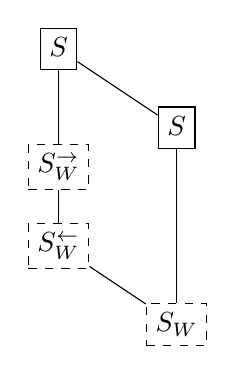
\begin{tikzpicture}
    \node (a1) at (0,3.5) [rectangle,draw] {$S_{\tyr}$};
    \node (a2) at (1.5,2.5) [rectangle,draw] {$S_{\tmr}$};
    \node (a3) at (0,2) [rectangle,draw,dashed] {$S_{\tyr W}^{\rightarrow}$};
    \node (a4) at (0,1) [rectangle,draw,dashed] {$S_{\tyr W}^{\leftarrow}$};
    \node (a5) at (1.5,0) [rectangle,draw,dashed] {$S_{\tmr W}$};
    \draw (a1) -- (a2);
    \draw (a2) -- (a5);
    \draw (a1) -- (a3);
    \draw (a3) -- (a4);
    \draw (a4) -- (a5);
  \end{tikzpicture}
  \vspace{-0.5em}
  \caption{Hierarchy of Context Schemas}
  \label{fig:ctxschema}
\end{wrapfigure}

The most interesting part of the Beluga development appears to be the particularly rich structure and interdependencies of the various schemas.
We would like to point out in particular, that while the schemas $S_{\tyr}$ and $S_{\tmr}$ could likely be inferred automatically by inspecting the involved type families, this does not appear to work for those schemas with auxiliary well-typedness assumptions (subscript $W$).
This contradicts the common belief that schema inference should in principle always be possible.

The schemas can be further arranged in a hierarchy (Figure~\ref{fig:ctxschema}).
A context satisfying $S_{\tyr}$ can always be weakened to one sitting lower in the hierarchy.
The hierarchy also induces a strengthening relationship, going upwards, as long as the subordination order of judgements under said contexts is respected.

%%% Local Variables:
%%% mode: latex
%%% TeX-master: "fscd17"
%%% End:
